\documentclass{article} % For LaTeX2e
\usepackage{hyperref}
\usepackage{url}
\usepackage[utf8]{inputenc}
\usepackage{amsmath}
\usepackage[numbers,sort]{natbib}
\usepackage{graphicx}
\usepackage[export]{adjustbox}
\usepackage{footmisc}
\usepackage[section]{placeins}
\usepackage{minted}
\usepackage{listings}
\usepackage{hyperref}
\DeclareGraphicsExtensions{.pdf,.png,.jpg,.eps}

\newlength\tindent
\setlength{\tindent}{\parindent}
\setlength{\parindent}{0pt}
\renewcommand{\indent}{\hspace*{\tindent}}


\author{
Gabriel C-Parent\\
}


\newcommand{\fix}{\marginpar{FIX}}
\newcommand{\new}{\marginpar{NEW}}

\begin{document}


\title{IFT6751: Homework 2}
      
\maketitle
\section{Introduction}

In this homework, two different approaches to solve the capacitated vehicle routing problem (CVRP) were designed. The first one is a genetic algorithm using specialized crossover and mutation operators whereas the the second one uses the Tabu Search to control local search with the $\lambda$-interchange neighbourhood.\newline

Two greedy local search methods are used within both methods to improve the results such as the 2-opt descent and  and the $\lambda$-interchange descent.\newline

Another method based on the Clark \& Wright savings is also used to initialize solutions for both metaheuristics.\newline


Both methods were tested against problem instances without length limit, from \citep{christofides} and compared to the best known solutions.\newline


A description of all the optimization methods along with special implementation details is given.
Some experimental results are then compared based on running time, implementation complexity and results quality.\newline

Finally, a user guide is given in the supplementary section \ref{user_guide}.



\newpage
\section{Local Search Methods}
\label{local_search}


\subsection{2-opt descent}
\label{local_tsp}

First, a simple and fast optimization method for the TSP was needed to improve the path of each routes.\newline

The local search method used to optimize individual routes is the steepest improvement method as described in \citep{steepest_improvement}.
Basically, it is an implementation of steepest descent implementation using the well known 2-opt operator.\newline

At each iteration, the best possible 2-opt is chosen, according to the reduction in total distance, until there isn't any possible improvement. The complexity of the procedure $O(n^{2})$ on the number of edges in the route.\newline

Although it might seem slow, usually the number of edges is quite small and the time spent optimizing routes is negligible.\newline



\subsection{$\lambda$-interchange descent}
\label{local_cluster}
Another optimization method was needed to exchange clients between routes, in this case the $\lambda$-interchange descent with $\lambda$=1 \citep{osman1993}.\newline

The possible transitions are the transfer of a client from a route to another and the swap of two clients between two routes. Since only feasible solutions are considered, only transitions that do not violate the capacity limit are considered.\newline

The procedure chooses the interchange with best possible improvement and applies it. Then the 2-opt descent is applied to the modified routes and the process is repeated until it gets stuck in a local minima.


\newpage
\section{Random Savings Initialization}
\label{random_savings}
The Clark \& Wright savings algorithm is a well known simple heuristic for the CVRP.
Many improvements were suggested for this heuristic \cite{clark_wright_ds}.\newline

The one used in this work is a slight variant of the parallel savings, where instead of choosing the best the best saving and merging the corresponding routes, the $k$ best savings are found and one is randomly chosen.\newline

This procedure is used in both the Tabu Search and Genetic Algorithm procedures.\newline

In the Genetic Algorithm procedure, the random savings is used to generate good initial solutions. The initialization step is costly but the quality of the initial population is great.\newline

In the Tabu Search procedure, the random savings is used to generate an initial solution and new solutions each time the patience threshold is reached.\newline

Random Savings itself is compared against both algorithm as a baseline.


\newpage
\section{Genetic Algorithm}
\label{genetic_algorithm}
%encodage d’une solution, sélection, croisement, mutation, remplacement de la population, critère d’arrêt

\subsection{Encoding}

The solutions are encoded using the route and solution objects. Basically, a route is a list of clients that starts at the depot and ends at the depot, where no client is repeated and the total capacity is lesser or equal to the vehicle capacity. A solution is a list of routes, where each client is in exactly one route.\newline

This representation isn't really friendly to classical genetic operators but allows functions defined on routes and solutions to be shared for both the Tabu Search and Genetic Algorithm representations.

\subsection{Objective Function}

The objective function is the minimization of the total distance of the routes.

\begin{equation*}
\begin{aligned}
& \text{minimize}
& & \sum\limits_{r \in solution} distance(r) \\
& \text{subject to}
& & weight(r) \leq vehicle\ capacity
\end{aligned}
\end{equation*}

\subsection{Selection}

The parents to the next generation are selected using the simple and well known binary tournament selection.


\subsection{Crossover}

The crossover used here can be explained in terms of the cluster-first route-second methods.\newline

Since the initial population is generated using the random savings \ref{random_savings} with 2-opt descent \ref{local_tsp} optimization applied on the resulting routes, the solutions are already good and the routes usually are pretty close to the best known solutions. However the choice of clusters, that is which clients belong together, is somewhat far from optimal.\newline

Therefore, what was needed was a crossover that would allow for new clusters to be created while using part of the routes of the parents. To do so, routes are selected from both parents and the remaining clients have routes assigned to them using the Clark \& Wright savings. The second part is where new clusters should be formed.


\subsubsection{Selection Of Inherited Routes}

In both parents, routes are sorted by the angle of their centroid (average of clients coordinates) relative to the depot and a quarter of the routes of each parents is selected so that overall about half the routes of the child will be inherited and the other half will be newly created in the second part.\newline

Let $n_1$ be the number of routes in the first parent. A contiguous sequence $\frac{n_1}{4}$ routes in selected in the first parent. Since they are sorted by their angle to the depot, the hope is that they are all very close to each other.\newline

In the second parents, only routes that share no clients with the selected routes from parent 1 are considered.  Obviously, it is possible that much less than $\frac{n_1}{4}$ remain and of those, at most $\frac{n_1}{4}$ hopefully contiguous routes are chosen using the same mechanism as for parent 1.\newline

Overall, at most $\frac{n_1}{2}$ routes are inherited.

\subsubsection{Assigning Routes To Remaining Clients}

Once the routes inherited are selected, the rest of the clients have routes assigned to them using the Clark \& Wright parallel savings. The path of each resulting routes is then improved using the 2-opt descent local search.


\subsection{Mutation}

A $n$ optimal $\lambda$-interchange \ref{local_cluster} with $\lambda$=1 are applied. In this case, $n$ is set to 5. That is $n$ iterations of the descent are done, unless a local optima is reached before.


\subsection{Population Swap}

An elitist population replacement is implemented. A fixed percentage of the best solutions is automatically inherited from the previous generation at each iteration.


\subsection{Stopping criteria}

A number of iterations is given.


\newpage
\section{Tabu Search}
\label{tabu_search}
%espace des solutions admissibles, fonction objectif, voisinage,
%liste tabou, critères d’aspiration, intensification, diversification, critère d’arrêt

With some variations, the Tabu Search implementation is very similar to the one described in \citep{osman1993}.


\subsection{Encoding}

The Tabu Search shares the same encoding for routes and solutions as the genetic algorithm. That way the local search methods are written once and work everywhere.

\subsection{Solution Space}

Only feasible solutions are considered, that is those not violating the capacity constraint.


\subsection{Objective Function}

The objective function is the minimization of the total distance of the routes. The same as the genetic algorithm.

\begin{equation*}
\begin{aligned}
& \text{minimize}
& & \sum\limits_{r \in solution} distance(r) \\
& \text{subject to}
& & weight(r) \leq vehicle\ capacity
\end{aligned}
\end{equation*}


\subsection{Neighbourhood Structure}

The neighbourhood of a solution is all the feasible non-tabu solutions that can be reached by applying the $\lambda$-interchange, with $\lambda$=1.\newline

The best attainable solution in the whole neighbourhood is chosen at each iteration.


\subsection{Tabu List}

The tabu list is implemented as a matrix keeping the expiration of tabu status for pairs of $(client, route)$. This is exactly the same as in \citep{osman1993}. A $null$ client is used to represent the interchanges that imply only one client.\newline

A fixed tabu duration is chosen according to the simple heuristic outlined in \citep{osman1993}, that is its value is
$max\{7,\ -40+9.6*ln(n * v)\}$
where $n$ is the number of clients and $v$ is the number of vehicles used in the initial solution.


\subsection{Asipration Criteria}
No aspiration criteria was used. A big improvement could probably come from having one.


\subsection{Intensification}
No intensification method was used.


\subsection{Diversification}

To allow for diversification, instead of keeping statistics on the solutions visited, a simple restart scheme was implemented.\newline

The tabu search algorithm takes an integer argument called $patience$. The $patience$ represents the number of iterations without new best solution found that is tolerated. If that number is crossed, the Tabu Search algorithm starts with a new solution and a fresh tabu list, procured by the random savings.


\subsection{Stopping Criteria}

As with the random savings, the stopping criteria can be a set number of iterations or a time limit, depending on the type of constraints the user has.\newline

For the experiment, a time limit of 60 seconds for each problem was used.


%------------------------------------------------------------------------------
\newpage
\section{Experimental Results}
\label{exp_results}

\subsection{Random Savings}

\begin{figure}[!htb]
\begin{center}
 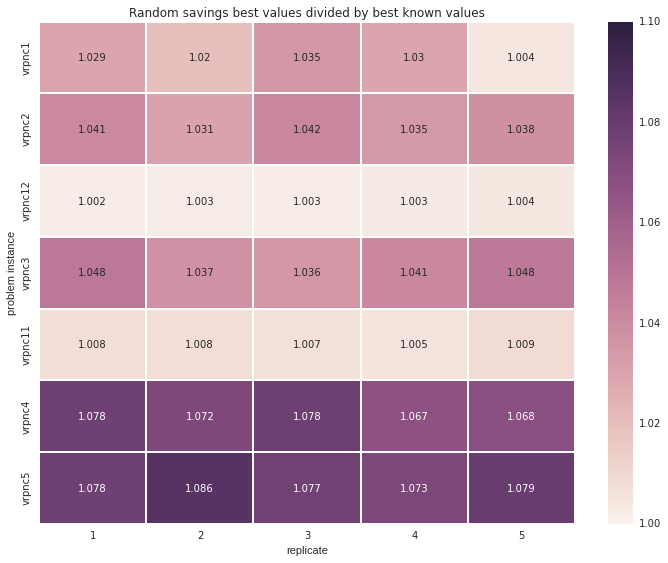
\includegraphics[scale=0.45]{figures/rs_best}
 \caption{\small The random savings algorithm is used to generate solutions for each problem instance. Each of the 5 replicates is a run of 60 seconds of generating solutions in a Monte Carlo fashion, whit a depth of 3 suboptimal choices considered (see \ref{random_savings} for more details). The total distance used by the best solution of each replicate is divided by the best known value of each problem instance. Seeing as each run lasts only 60 seconds, the results are surprisingly good.}
 \label{rs_fig}
 \end{center}
\end{figure}


\newpage
\subsection{Genetic Algorithm}

\begin{figure}[!htb]
\begin{center}
 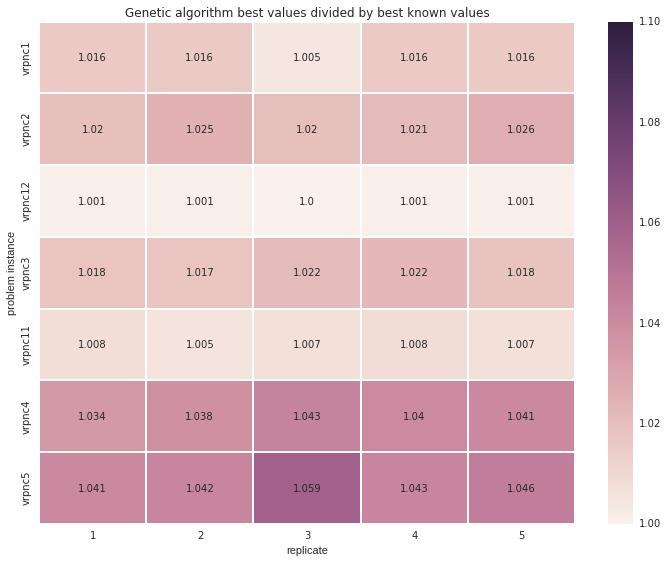
\includegraphics[scale=0.45]{figures/ga_best}
 \caption{\small  The genetic algorithm is used to generate solutions for each problem instance. Each of the 5 replicates is a run of 100 iterations with a population size of 200. The average time for each problem is specified on the $y$ axis. Additional parameters are specified in the corresponding IPython notebook. With 5 replicates, the total distance used by the best solution of each replicate is divided by the best known value of each problem instance. The results are acceptable, but not as good as expected given that the random savings was much quicker and the solutions generated here are only slightly better. Then again, the last bits of performance are usually the hardest to get.}
 \label{ga_fig}
 \end{center}
\end{figure}


\newpage
\subsection{Tabu Search}

\begin{figure}[!htb]
\begin{center}
 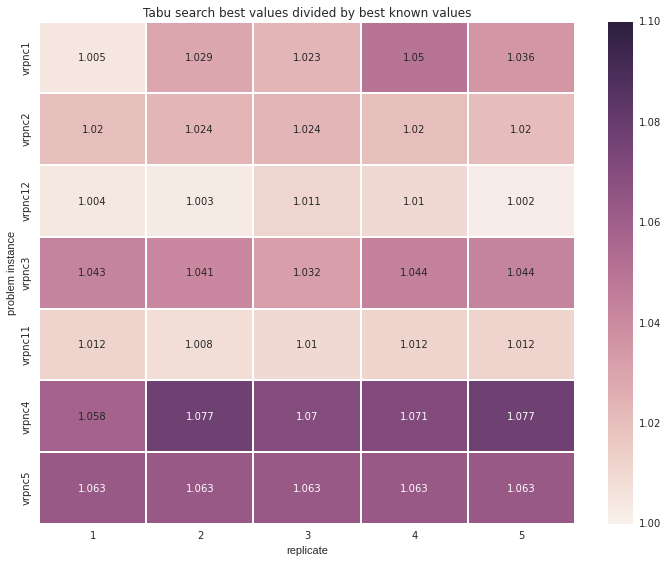
\includegraphics[scale=0.45]{figures/tabu_search}
 \caption{\small  The Tabu Search is used to generate solutions for each problem instance. Each of the 5 replicates is a run of 60 seconds with a patience of 1000 iterations. Additional parameters are specified in the corresponding IPython notebook. With 5 replicates, the total distance used by the best solution of each replicate is divided by the best known value of each problem instance. The results are quite good, but far from the best known values and sadly too close to the random savings to justify the complexity of the implementation. Given more time, much better results could probably have been reached.}
 \label{ts_fig}
 \end{center}
\end{figure}


\newpage
\section{Discussion}
\label{analysis_results}

The CVRP is a hard problem and the experimental results are acceptable in my opinion.\newline

\subsection{Random Savings: Speed And Simplicity}
The Random Savings \ref{rs_fig} had much more success than expected, especially since there was a 30 seconds time limit for solving. For vrpnc1, vrpnc12 and vrpnc11 the best results are very close to optimality. This can be explained by the location of the clients for vrpnc11 and vrpnc12 while vrpnc1 has the least amount of clients.\newline

Overall the simplicity of implementation and speed of solving made this algorithm very interesting. That is why both the Genetic Algorithm and Tabu Search solvers use it for different roles.



\subsection{Genetic Algorithm: Modularity}

The Genetic Algorithm managed to improve quite a lot the initial solutions generated by the random savings.
The algorithm is time consuming but the results achieved are interesting, although not as good as the best known values.\newline

The implementation of the genetic algorithm more modular than the Tabu Search and as such allowed for many options of crossover and mutation operators to be tried.\newline


In my opinion, this algorithm was simpler and much more fun to implement than the Tabu Search.


\subsection{Tabu Search: Middle Ground}

The tabu search was quite hard to implement compared to previous algorithms. In my opinion it would be because all of the design parameters must be known beforehand to make it efficient. The choice of the local optimization method is crucial dictates how the rest of the algorithm should be implemented more strictly than I would like.\newline

However, since the best known values have been obtained using such algorithm, the idea have its merits.\newline

With this implementation and a runtime limit of a minute for each program, the results stand in between the random savings and the genetic algorithm in terms of solution quality.\newline

The simplicity of the implementation is probably to blame for the relatively poor performance.


\subsection{Tradeoffs}

Considering three attributes, that is speed, simplicity and quality of the solutions, each algorithm has something interesting to offer.\newline


\subsubsection{Simplicity}

From the standpoint of simplicity, the random savings is a clear winner. With only 140 lines of code, a relatively efficient implementation of it could be done. Second would be the genetic algorithm with 183 lines of code and finally the tabu solver with 253 lines of code. Although simply counting lines is not suitable proof of simplicity, in this case I think it correlates pretty well.\newline


\subsubsection{Solution Quality}

Since the genetic algorithm is given much more time than the two others, it is no surprise that it has the best solution quality. Second comes the tabu search and then the random savings.\newline

In my opinion, the tabu search has a lot more to offer than what I implemented, but I was limited by my actual knowledge. I would initially have liked to implement something like the TabuRoute algorithm \citep{taburoute}, but the heavy dependency on previous work and the lack of example implementations was discouraging.\newline


\subsubsection{Speed}

In my opinion, considering the time limit imposed on Tabu Search and the relatively poor implementation, I would declare the Tabu Search the best in regard of speed. I believe that given a little more time it would probably outshine both the genetic algorithm and random savings.\newline

The random savings would rank second and the genetic algorithm far last.


\section{Conclusion}

Overall, this homework was an interesting exercise and I tried to come up with original solutions to solve the capacitated vehicle routing problem.\newline

Quite a lot of literature was explored to come up with solutions, but sadly most of the solutions I came upon depended on earlier articles inaccessible because of paywalls and very few (read none) had exemple implementations. I would honestly have preferred a Fortran code to the pseudocode given.\newline

None of the solvers got really close to the results given by TabuRoute \citep{taburoute} but then again, I didn't expect them to be that good.\newline


\bibliographystyle{plain}

\bibliography{dev2}


\newpage
\section{Supplementary Materials}

\subsection{User Guide}
\label{user_guide}

The following section should help with verification of the results and repeatability.\newline

The language used is a mix of python and cython, an optimising compiler that allows static typing and generates C code.


\subsubsection{Working Environment}
All computational results obtained in this work should be repeatable given a suitable python environment. The particular dependencies of this work are the Cython, Numpy, IPython and Seaborn along with standard python environment.\newline

The following python environment was used:

\begin{verbatim}
CPython 2.7.9
ipython 2.2.0

numpy 1.9.2
cython 0.21
ipython 2.2.0
seaborn 0.5.1

compiler   : GCC 4.4.7 20120313 (Red Hat 4.4.7-1)
system     : Linux
release    : 3.13.0-46-generic
machine    : x86_64
processor  : x86_64
CPU cores  : 4
interpreter: 64bit

\end{verbatim}

As of now, my personal recommendation is to use the excellent \href{http://continuum.io/downloads}{Anaconda python distribution} from Continuum Analytics.


\subsubsection{Running Computational Results}

All computational results and figures are contained in the form of IPython Notebooks with the hope of allowing repeatability and reproducibility.


If IPython is available on the computer, an IPython Notebook service can be launched from command line using the following call.

\begin{minted}[mathescape,
               numbersep=5pt,
               framesep=2mm]{bash}
ipython notebook    
\end{minted}

This allows viewing and recomputation of the results.\newline


Alternatively, the IPython notebooks can be viewed online if it is reachable from a url using the \href{http://nbviewer.IPython.org/}{nbviewer tool}. This allows viewing a static version of an IPython Notebook.



\newpage
\subsection{Experimental Solutions}
Here are the resulting solutions for each problem. The depot is represented using the index 0. All routes start and end at the depot. A list of routes is considered a solution and the total length of the routes is also given.


\subsubsection{Random Savings}
\begin{lstlisting}[breaklines, basicstyle=\tiny]
vrpnc1
distance 526.926289575
[
[0, 8, 26, 31, 28, 3, 36, 35, 20, 22, 1, 32, 0]
[0, 12, 37, 44, 15, 45, 33, 39, 10, 49, 5, 46, 0]
[0, 6, 14, 25, 24, 43, 7, 23, 48, 27, 0]
[0, 38, 9, 16, 50, 30, 34, 21, 29, 2, 11, 0]
[0, 47, 4, 17, 42, 19, 40, 41, 13, 18, 0]
]

vrpnc2
distance 854.232620565
[
[0, 2, 28, 61, 22, 62, 73, 33, 0]
[0, 12, 72, 39, 9, 31, 10, 58, 0]
[0, 51, 3, 44, 32, 40, 17, 26, 0]
[0, 37, 20, 70, 60, 71, 69, 36, 47, 21, 74, 0]
[0, 35, 53, 11, 66, 65, 38, 0]
[0, 50, 25, 55, 18, 24, 49, 16, 6, 68, 0]
[0, 52, 27, 13, 54, 19, 59, 14, 0]
[0, 63, 23, 56, 41, 64, 42, 43, 1, 0]
[0, 67, 7, 8, 46, 34, 4, 0]
[0, 75, 30, 48, 5, 15, 57, 29, 45, 0]
]

vrpnc12
distance 819.597073863
[
[0, 5, 3, 7, 8, 11, 9, 6, 4, 2, 1, 75, 0]
[0, 13, 17, 18, 19, 15, 16, 14, 12, 10, 0]
[0, 21, 23, 26, 28, 30, 29, 27, 25, 24, 22, 20, 0]
[0, 32, 33, 31, 35, 37, 38, 39, 36, 34, 0]
[0, 43, 42, 41, 40, 44, 46, 45, 48, 51, 50, 52, 49, 47, 0]
[0, 57, 55, 54, 53, 56, 58, 60, 59, 0]
[0, 81, 78, 76, 71, 70, 73, 77, 79, 80, 72, 61, 64, 68, 69, 0]
[0, 67, 65, 63, 74, 62, 66, 0]
[0, 90, 87, 86, 83, 82, 84, 85, 88, 89, 91, 0]
[0, 99, 100, 97, 93, 92, 94, 95, 96, 98, 0]
]

vrpnc3
distance 856.169048665
[
[0, 28, 76, 77, 3, 68, 80, 29, 24, 55, 25, 4, 54, 12, 26, 0]
[0, 40, 73, 22, 41, 23, 67, 39, 56, 75, 74, 72, 21, 0]
[0, 50, 33, 81, 9, 51, 20, 66, 65, 71, 35, 34, 78, 79, 0]
[0, 52, 31, 10, 63, 90, 32, 30, 70, 1, 69, 27, 0]
[0, 60, 5, 84, 61, 16, 44, 14, 38, 86, 17, 45, 83, 18, 0]
[0, 13, 94, 95, 87, 42, 43, 15, 57, 2, 58, 53, 0]
[0, 88, 62, 48, 47, 19, 11, 64, 49, 36, 46, 8, 82, 7, 0]
[0, 97, 92, 59, 98, 37, 100, 91, 85, 93, 99, 96, 6, 89, 0]
]

vrpnc11
distance 1046.04909402
[
[0, 2, 1, 3, 4, 5, 6, 7, 9, 10, 11, 15, 14, 13, 12, 8, 0]
[0, 17, 16, 19, 25, 22, 24, 27, 30, 33, 34, 36, 29, 32, 35, 31, 28, 26, 23, 20, 21, 109, 0]
[0, 37, 38, 39, 42, 41, 44, 47, 46, 49, 50, 51, 48, 45, 43, 40, 101, 0]
[0, 95, 102, 105, 106, 107, 104, 103, 99, 100, 116, 115, 97, 94, 96, 93, 92, 89, 87, 0]
[0, 98, 68, 73, 76, 77, 79, 80, 78, 72, 75, 74, 71, 70, 69, 67, 0]
[0, 110, 52, 54, 57, 59, 65, 61, 62, 64, 66, 63, 60, 56, 58, 55, 53, 0]
[0, 120, 119, 81, 112, 84, 117, 113, 83, 108, 118, 18, 114, 90, 91, 85, 86, 111, 82, 88, 0]
]

vrpnc4
distance 1083.02571683
[
[0, 48, 47, 124, 46, 36, 143, 49, 64, 11, 107, 19, 123, 7, 0]
[0, 13, 95, 92, 98, 37, 100, 85, 93, 59, 104, 99, 96, 0]
[0, 18, 106, 82, 114, 8, 45, 125, 83, 60, 118, 5, 0]
[0, 27, 132, 31, 127, 52, 146, 112, 0]
[0, 28, 12, 150, 80, 68, 121, 29, 24, 134, 130, 54, 109, 138, 0]
[0, 50, 51, 103, 9, 120, 135, 35, 136, 65, 71, 66, 128, 20, 0]
[0, 53, 23, 67, 39, 139, 25, 55, 4, 110, 149, 26, 0]
[0, 69, 1, 101, 70, 122, 30, 131, 32, 90, 63, 126, 108, 10, 62, 148, 88, 0]
[0, 84, 17, 113, 86, 140, 38, 14, 119, 44, 141, 16, 61, 91, 6, 0]
[0, 89, 147, 94, 117, 97, 42, 142, 43, 15, 57, 144, 87, 137, 0]
[0, 76, 116, 77, 3, 79, 129, 78, 34, 81, 33, 102, 111, 0]
[0, 105, 40, 21, 73, 72, 56, 75, 74, 133, 22, 41, 145, 115, 2, 58, 0]
]

vrpnc5
distance 1373.17238242
[
[0, 6, 96, 61, 16, 141, 38, 140, 86, 113, 17, 173, 84, 5, 0]
[0, 21, 197, 56, 186, 23, 67, 170, 39, 139, 187, 25, 55, 165, 0]
[0, 27, 132, 176, 1, 162, 31, 190, 127, 167, 146, 0]
[0, 40, 180, 198, 110, 4, 155, 179, 130, 54, 154, 138, 0]
[0, 50, 102, 157, 51, 9, 81, 33, 185, 79, 3, 158, 77, 0]
[0, 156, 112, 13, 152, 58, 53, 105, 28, 111, 0]
[0, 69, 101, 70, 30, 160, 131, 32, 181, 63, 126, 90, 108, 10, 189, 0]
[0, 76, 196, 116, 184, 12, 80, 150, 177, 109, 195, 149, 26, 0]
[0, 94, 183, 147, 89, 0]
[0, 117, 97, 151, 92, 59, 98, 37, 100, 193, 91, 85, 93, 99, 104, 0]
[0, 122, 128, 20, 188, 66, 71, 65, 136, 35, 135, 161, 103, 0]
[0, 46, 124, 168, 47, 36, 143, 49, 64, 11, 175, 107, 19, 123, 7, 52, 0]
[0, 137, 87, 172, 144, 57, 15, 43, 42, 142, 14, 192, 119, 44, 191, 95, 0]
[0, 153, 106, 194, 82, 48, 182, 62, 159, 148, 88, 0]
[0, 129, 120, 164, 34, 78, 169, 121, 29, 24, 163, 134, 68, 0]
[0, 166, 118, 60, 83, 199, 125, 45, 174, 8, 114, 18, 0]
[0, 2, 178, 115, 145, 41, 22, 133, 75, 74, 171, 72, 73, 0]
]
\end{lstlisting}


\newpage
\subsubsection{Genetic Algorithm}
\begin{lstlisting}[breaklines, basicstyle=\tiny]

vrpnc1
distance 531.024872236
[
[0, 1, 22, 31, 28, 3, 36, 35, 20, 29, 2, 32, 0]
[0, 6, 14, 24, 43, 23, 7, 26, 8, 48, 27, 0]
[0, 12, 38, 9, 30, 34, 21, 50, 16, 11, 0]
[0, 47, 17, 37, 44, 15, 45, 33, 39, 10, 49, 5, 46, 0]
[0, 4, 42, 19, 40, 41, 13, 25, 18, 0]
[0, 0]
]

vrpnc2
distance 843.093409675
[
[0, 51, 3, 44, 32, 9, 39, 72, 58, 0]
[0, 10, 31, 55, 25, 50, 18, 24, 49, 0]
[0, 73, 43, 42, 64, 41, 56, 23, 63, 16, 0]
[0, 30, 48, 47, 21, 74, 2, 68, 0]
[0, 29, 5, 36, 69, 71, 60, 70, 20, 37, 15, 57, 0]
[0, 4, 45, 27, 52, 46, 34, 0]
[0, 6, 33, 1, 22, 61, 28, 62, 0]
[0, 7, 35, 14, 59, 19, 54, 13, 8, 0]
[0, 53, 11, 66, 65, 38, 0]
[0, 17, 40, 12, 26, 67, 75, 0]
]

vrpnc12
distance 820.227590565
[
[0, 57, 55, 54, 53, 56, 58, 60, 59, 0]
[0, 66, 62, 74, 63, 65, 67, 0]
[0, 5, 3, 7, 8, 11, 9, 6, 4, 2, 1, 75, 0]
[0, 10, 12, 14, 16, 15, 19, 18, 17, 13, 0]
[0, 20, 24, 25, 27, 29, 30, 28, 26, 23, 22, 21, 0]
[0, 34, 36, 39, 38, 37, 35, 31, 33, 32, 0]
[0, 43, 41, 40, 42, 44, 46, 45, 48, 51, 50, 52, 49, 47, 0]
[0, 81, 78, 76, 71, 70, 73, 77, 79, 80, 72, 61, 64, 68, 69, 0]
[0, 91, 89, 88, 85, 84, 82, 83, 86, 87, 90, 0]
[0, 98, 96, 95, 94, 92, 93, 97, 100, 99, 0]
]

vrpnc3
distance 842.036213898
[
[0, 1, 51, 9, 81, 33, 78, 34, 35, 71, 65, 66, 20, 30, 70, 69, 0]
[0, 27, 31, 10, 32, 90, 63, 64, 49, 19, 11, 62, 88, 52, 0]
[0, 13, 97, 87, 42, 43, 15, 57, 41, 22, 74, 72, 73, 21, 40, 53, 0]
[0, 26, 54, 4, 55, 25, 39, 67, 23, 56, 75, 2, 58, 0]
[0, 50, 76, 77, 3, 79, 29, 24, 68, 80, 12, 28, 0]
[0, 18, 60, 83, 8, 82, 7, 48, 47, 36, 46, 45, 17, 84, 5, 89, 0]
[0, 6, 96, 99, 93, 59, 95, 94, 0]
[0, 98, 85, 61, 16, 86, 38, 14, 44, 91, 100, 37, 92, 0]
]

vrpnc11
distance 1047.18488127
[
[0, 8, 12, 13, 14, 15, 11, 10, 9, 7, 6, 5, 4, 3, 1, 2, 88, 0]
[0, 17, 16, 19, 22, 24, 25, 28, 27, 33, 30, 31, 34, 36, 35, 32, 29, 26, 23, 20, 21, 109, 0]
[0, 100, 53, 55, 58, 56, 60, 63, 66, 64, 62, 61, 65, 59, 57, 54, 52, 0]
[0, 119, 81, 112, 85, 84, 117, 113, 83, 108, 118, 18, 114, 90, 91, 89, 92, 87, 0]
[0, 98, 68, 73, 76, 77, 79, 80, 78, 75, 72, 74, 71, 70, 69, 67, 0]
[0, 110, 40, 43, 45, 48, 51, 50, 49, 47, 46, 44, 41, 42, 39, 38, 37, 0]
[0, 82, 111, 86, 95, 102, 101, 99, 96, 93, 94, 97, 115, 116, 103, 104, 107, 106, 105, 120, 0]
]

vrpnc4
distance 1054.66014431
[
[0, 111, 76, 116, 77, 3, 121, 29, 24, 134, 150, 80, 68, 12, 0]
[0, 79, 129, 78, 34, 35, 135, 9, 120, 81, 33, 102, 50, 0]
[0, 27, 69, 101, 70, 30, 20, 128, 66, 65, 136, 71, 103, 51, 122, 1, 132, 0]
[0, 96, 104, 99, 59, 93, 85, 91, 100, 98, 37, 92, 95, 0]
[0, 13, 137, 144, 57, 15, 43, 142, 42, 87, 97, 117, 94, 6, 147, 89, 0]
[0, 40, 21, 73, 72, 74, 75, 133, 22, 41, 145, 115, 2, 58, 112, 0]
[0, 110, 4, 56, 23, 67, 39, 139, 25, 55, 130, 54, 109, 138, 0]
[0, 18, 106, 82, 114, 8, 125, 45, 84, 5, 118, 60, 0]
[0, 7, 123, 19, 107, 11, 64, 49, 143, 36, 47, 46, 124, 48, 0]
[0, 127, 31, 10, 108, 131, 32, 90, 63, 126, 62, 148, 88, 52, 146, 0]
[0, 61, 16, 141, 44, 119, 14, 38, 140, 86, 113, 17, 83, 0]
[0, 53, 105, 149, 26, 28, 0]
]

vrpnc5
distance 1345.27517451
[
[0, 2, 178, 57, 15, 43, 142, 42, 172, 144, 87, 97, 117, 94, 183, 0]
[0, 152, 58, 112, 156, 0]
[0, 53, 73, 171, 74, 75, 56, 186, 23, 133, 22, 41, 145, 115, 137, 0]
[0, 26, 149, 179, 110, 155, 4, 197, 72, 198, 180, 105, 0]
[0, 1, 122, 30, 20, 188, 66, 128, 160, 131, 32, 70, 101, 162, 0]
[0, 127, 148, 62, 159, 126, 63, 181, 90, 108, 10, 189, 69, 132, 0]
[0, 52, 106, 194, 182, 88, 31, 190, 167, 27, 0]
[0, 146, 7, 123, 19, 107, 175, 11, 64, 49, 143, 36, 47, 168, 124, 46, 0]
[0, 77, 3, 158, 121, 29, 24, 163, 134, 68, 80, 150, 177, 109, 12, 0]
[0, 89, 166, 60, 118, 84, 17, 113, 61, 173, 5, 104, 99, 147, 0]
[0, 6, 16, 86, 140, 38, 14, 192, 119, 44, 141, 191, 91, 193, 0]
[0, 153, 82, 48, 114, 8, 174, 45, 125, 199, 83, 18, 0]
[0, 50, 157, 33, 81, 120, 164, 34, 78, 169, 129, 79, 185, 0]
[0, 195, 54, 130, 165, 55, 25, 170, 67, 39, 187, 139, 21, 40, 0]
[0, 28, 154, 138, 184, 116, 196, 76, 111, 0]
[0, 102, 9, 135, 35, 136, 65, 71, 161, 103, 51, 176, 0]
[0, 13, 95, 151, 92, 37, 98, 100, 85, 93, 59, 96, 0]
]
\end{lstlisting}

\newpage
\subsubsection{Tabu Search}
\begin{lstlisting}[breaklines, basicstyle=\tiny]
vrpnc1
distance 527.032223504
[
[0, 0]
[0, 32, 1, 22, 20, 35, 36, 3, 28, 31, 26, 8, 0]
[0, 46, 5, 49, 10, 39, 33, 45, 15, 44, 37, 12, 0]
[0, 18, 13, 41, 40, 19, 42, 17, 4, 47, 0]
[0, 27, 48, 23, 7, 43, 24, 25, 14, 6, 0]
[0, 38, 9, 30, 34, 21, 50, 16, 29, 2, 11, 0]
]

vrpnc2
distance 852.043752574
[
[0, 3, 44, 50, 25, 55, 18, 24, 49, 16, 0]
[0, 0]
[0, 34, 46, 52, 27, 45, 4, 0]
[0, 7, 53, 14, 59, 19, 54, 8, 0]
[0, 35, 11, 66, 65, 38, 58, 0]
[0, 13, 57, 15, 20, 70, 60, 71, 69, 21, 74, 0]
[0, 33, 62, 22, 61, 28, 2, 68, 0]
[0, 75, 67, 26, 12, 40, 17, 0]
[0, 51, 32, 9, 39, 31, 10, 72, 0]
[0, 73, 1, 43, 42, 64, 41, 56, 23, 63, 0]
[0, 29, 5, 37, 36, 47, 48, 30, 6, 0]
]

vrpnc12
distance 821.152127551
[
[0, 75, 1, 2, 4, 6, 9, 11, 8, 7, 5, 0]
[0, 10, 12, 14, 16, 15, 19, 18, 17, 13, 0]
[0, 20, 24, 25, 27, 29, 30, 28, 26, 23, 22, 21, 0]
[0, 34, 36, 39, 38, 37, 35, 31, 33, 32, 0]
[0, 47, 49, 52, 50, 51, 48, 45, 46, 44, 42, 40, 41, 43, 0]
[0, 57, 55, 54, 53, 56, 58, 60, 59, 0]
[0, 67, 65, 63, 74, 62, 66, 0]
[0, 69, 68, 64, 61, 72, 80, 79, 77, 73, 70, 71, 76, 78, 81, 0]
[0, 90, 87, 86, 83, 82, 84, 85, 88, 89, 91, 0]
[0, 98, 96, 95, 94, 92, 93, 97, 100, 99, 3, 0]
]

vrpnc3
distance 852.78030111
[
[0, 13, 87, 97, 59, 94, 0]
[0, 27, 31, 10, 62, 11, 19, 47, 48, 7, 88, 52, 0]
[0, 82, 46, 36, 49, 64, 63, 90, 32, 66, 65, 71, 20, 30, 70, 69, 0]
[0, 53, 58, 21, 73, 72, 74, 75, 56, 4, 54, 26, 0]
[0, 28, 76, 77, 3, 79, 78, 34, 35, 9, 51, 81, 33, 50, 1, 0]
[0, 40, 22, 41, 23, 67, 39, 25, 55, 24, 29, 68, 80, 12, 0]
[0, 89, 18, 60, 83, 8, 45, 17, 84, 5, 61, 85, 93, 99, 96, 6, 0]
[0, 95, 92, 98, 37, 100, 91, 16, 86, 38, 44, 14, 43, 15, 42, 57, 2, 0]
]

vrpnc11
distance 1050.25117554
[
[0, 17, 16, 19, 25, 22, 24, 27, 33, 30, 31, 34, 36, 29, 35, 32, 28, 26, 23, 20, 21, 109, 0]
[0, 101, 40, 43, 45, 48, 51, 50, 49, 46, 47, 44, 42, 41, 37, 38, 39, 0]
[0, 87, 91, 90, 114, 18, 118, 108, 83, 113, 117, 84, 112, 81, 82, 119, 120, 0]
[0, 88, 2, 1, 3, 4, 10, 11, 15, 14, 13, 12, 8, 9, 7, 6, 5, 0]
[0, 95, 102, 105, 106, 107, 104, 103, 99, 100, 116, 115, 97, 94, 96, 93, 92, 89, 85, 86, 111, 0]
[0, 98, 68, 73, 76, 77, 79, 80, 78, 72, 75, 74, 71, 70, 69, 67, 0]
[0, 110, 52, 54, 57, 59, 65, 61, 62, 64, 66, 63, 60, 56, 58, 55, 53, 0]
]

vrpnc4
distance 1088.32335076
[
[0, 26, 149, 21, 73, 72, 74, 75, 133, 22, 41, 145, 58, 0]
[0, 33, 81, 120, 9, 103, 71, 65, 136, 35, 135, 34, 78, 129, 76, 0]
[0, 82, 47, 36, 143, 49, 64, 63, 126, 11, 107, 19, 123, 0]
[0, 147, 83, 114, 8, 125, 45, 46, 124, 48, 7, 106, 52, 0]
[0, 116, 77, 3, 79, 121, 29, 24, 134, 80, 150, 68, 12, 138, 0]
[0, 105, 40, 115, 2, 144, 57, 15, 43, 142, 42, 87, 137, 0]
[0, 132, 69, 1, 20, 66, 128, 131, 32, 90, 108, 10, 62, 148, 88, 0]
[0, 89, 5, 84, 17, 113, 86, 140, 38, 14, 100, 37, 13, 0]
[0, 6, 96, 93, 85, 61, 16, 141, 44, 119, 91, 98, 92, 97, 117, 0]
[0, 53, 110, 4, 56, 23, 67, 39, 139, 25, 55, 130, 54, 109, 0]
[0, 127, 31, 101, 70, 30, 122, 51, 102, 50, 111, 28, 0]
[0, 27, 146, 18, 60, 118, 104, 99, 59, 95, 94, 112, 0]
]

vrpnc5
distance 1372.80329495
[
[0, 10, 189, 108, 131, 32, 90, 126, 63, 181, 64, 49, 143, 36, 0]
[0, 2, 178, 115, 73, 72, 197, 155, 4, 110, 198, 180, 0]
[0, 138, 154, 68, 116, 196, 184, 0]
[0, 147, 118, 83, 199, 125, 45, 174, 8, 114, 0]
[0, 60, 84, 17, 113, 86, 140, 38, 44, 119, 192, 14, 142, 13, 0]
[0, 88, 148, 159, 62, 182, 194, 106, 153, 18, 166, 89, 0]
[0, 81, 164, 120, 9, 161, 71, 103, 51, 122, 1, 0]
[0, 82, 48, 124, 46, 47, 168, 19, 107, 175, 11, 123, 7, 52, 146, 0]
[0, 50, 102, 157, 33, 185, 79, 129, 169, 29, 121, 3, 158, 77, 76, 0]
[0, 183, 94, 59, 93, 85, 98, 151, 95, 0]
[0, 87, 172, 42, 43, 15, 41, 22, 133, 75, 74, 171, 145, 57, 144, 137, 0]
[0, 78, 34, 135, 35, 136, 65, 66, 188, 20, 128, 160, 30, 70, 101, 0]
[0, 109, 165, 55, 25, 170, 187, 139, 39, 67, 23, 186, 56, 21, 40, 0]
[0, 12, 177, 150, 80, 163, 24, 134, 54, 130, 179, 195, 149, 26, 0]
[0, 27, 167, 127, 190, 31, 162, 69, 132, 176, 111, 28, 0]
[0, 117, 97, 92, 37, 100, 193, 91, 191, 141, 16, 61, 173, 5, 99, 104, 96, 6, 0]
[0, 53, 105, 58, 152, 112, 156, 0]
]
\end{lstlisting}



\end{document}


